\subsection{Creative Commons Gadget}

\subsubsection{Introduction}
The default license for any creation of any kind is the restrictive copyright. Copyright tries to ensure that all the rights remain to the original author of the content, but sometimes it can be advantageous to let people freely or semi-freely use, distribute or modify the content. One of the most popular, with over 400 million \cite{ref:the_power_of_open}, are the Creative Commons set of licenses. These are not adecuate for licensing software, but in the context of Wave the content is usually creative work, for which Creative Commons makes a good job.

\subsubsection{State of the Art}
Wave doesnt have any way of publishing your content under any specific license. Kune has the option for publishing Waves in your personal space under one of the existing Creative Commons Licenses. Outside of the personal space, Kune preserves Wave's aspect and removes the space where the license is in the personal space, so no license is imposed to other participants in a wave.

\subsubsection{Results}
This extension allows participants to set a Creative Commons license to a specific blip, by inserting a gadget in the content and answering questions to reach the adequate license that meets the requierements. The Figure \ref{fig:cc_gadget} shows the final result of this extension.

\begin{figure}[h]
  \center
    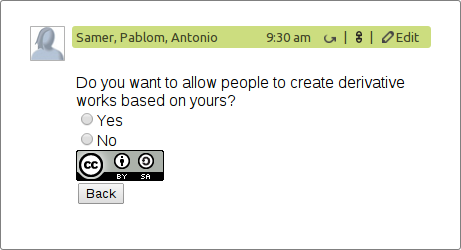
\includegraphics[keepaspectratio, scale=0.7]{Media/Captures/Extensions/CCGadget.png}
  \caption{Creative Commons Gadget}
  \label{fig:cc_gadget}
\end{figure}

